\clearpage 

\section{Discrete To Continuous Time}

\begin{tcolorbox}	
	\begin{tabular}{p{2.75cm} p{0.2cm} p{10.5cm}} 	
		\textbf{Header File}   &:& discrete\_to\_continuous\_time.h \\
		\textbf{Source File}   &:& discrete\_to\_continuous\_time.cpp \\
		\textbf{Version}  &:& 20180815(Filipa Simoes) \\
	\end{tabular}
\end{tcolorbox}

This block allows the conversion of a signal discrete in time to a continuous signal in time.

\subsection*{Input Signals}
Sequence of 1 and -1;
Number: 1 [S2 or S3]);
Type: Discrete Time and Discrete Amplitude;

\subsection*{Input Parameters}

Number of samples per Symbol (default:8; Type: int);

\subsection*{Output Signals}
Sequence of Dirac delta functions;
Number:1 [S4 or S5];
Type: Continuous Time and Discrete Amplitude;



%\begin{table}[h]
	%\centering
	%\begin{tabular}{|c|c|c|c|cccc}
		%\cline{1-4}
		%\textbf{Parameter} & \textbf{Type} & \textbf{Values} &   \textbf{Default}& \\ \cline{1-4}
		%numberOfSamplesPerSymbol & int & any & $8$ \\ \cline{1-4}
	%\end{tabular}
	%\caption{Binary source input parameters}
	%\label{table:disc2cont_in_par}
%\end{table}

%\begin{itemize}
%	\item numberOfSamplesPerSymbol\{8\} \linebreak
%	(int)
%\end{itemize}

%%\subsection*{Methods}

%%DiscreteToContinuousTime(vector$<$Signal *$>$ \&inputSignals, vector$<$Signal *$>$ %%\&outputSignals) :Block(inputSignals, outputSignals)\{\};
%%\bigbreak	
%%void initialize(void);
%%\bigbreak	
%%bool runBlock(void);
%%\bigbreak	
%%void setNumberOfSamplesPerSymbol(int nSamplesPerSymbol)
%%\bigbreak
%%int const getNumberOfSamplesPerSymbol(void)


\subsection*{Functional Description}
Reads the input signal buffer value, puts it in the output signal buffer;
Fills the space available for that symbol with zeros;
NumberOfSamplesPerSymbol:  space available in the buffer for each symbol.

\subsection*{Example}

For a binary source output: 01001010111001101000100111100010 \\
M-QAM MAPPER output(Timetocontinuous Input): \\
S1(I): -1;1;1;1;-1;1;-1;1;1;1;1;-1;-1;1;1;1;1\\
S2(Q): 1;1;-1;-1;-1;-1;1;-1;-1;1;-1;1;-1;-1;1;-1\\
		
\begin{figure}[h]
	\centering
	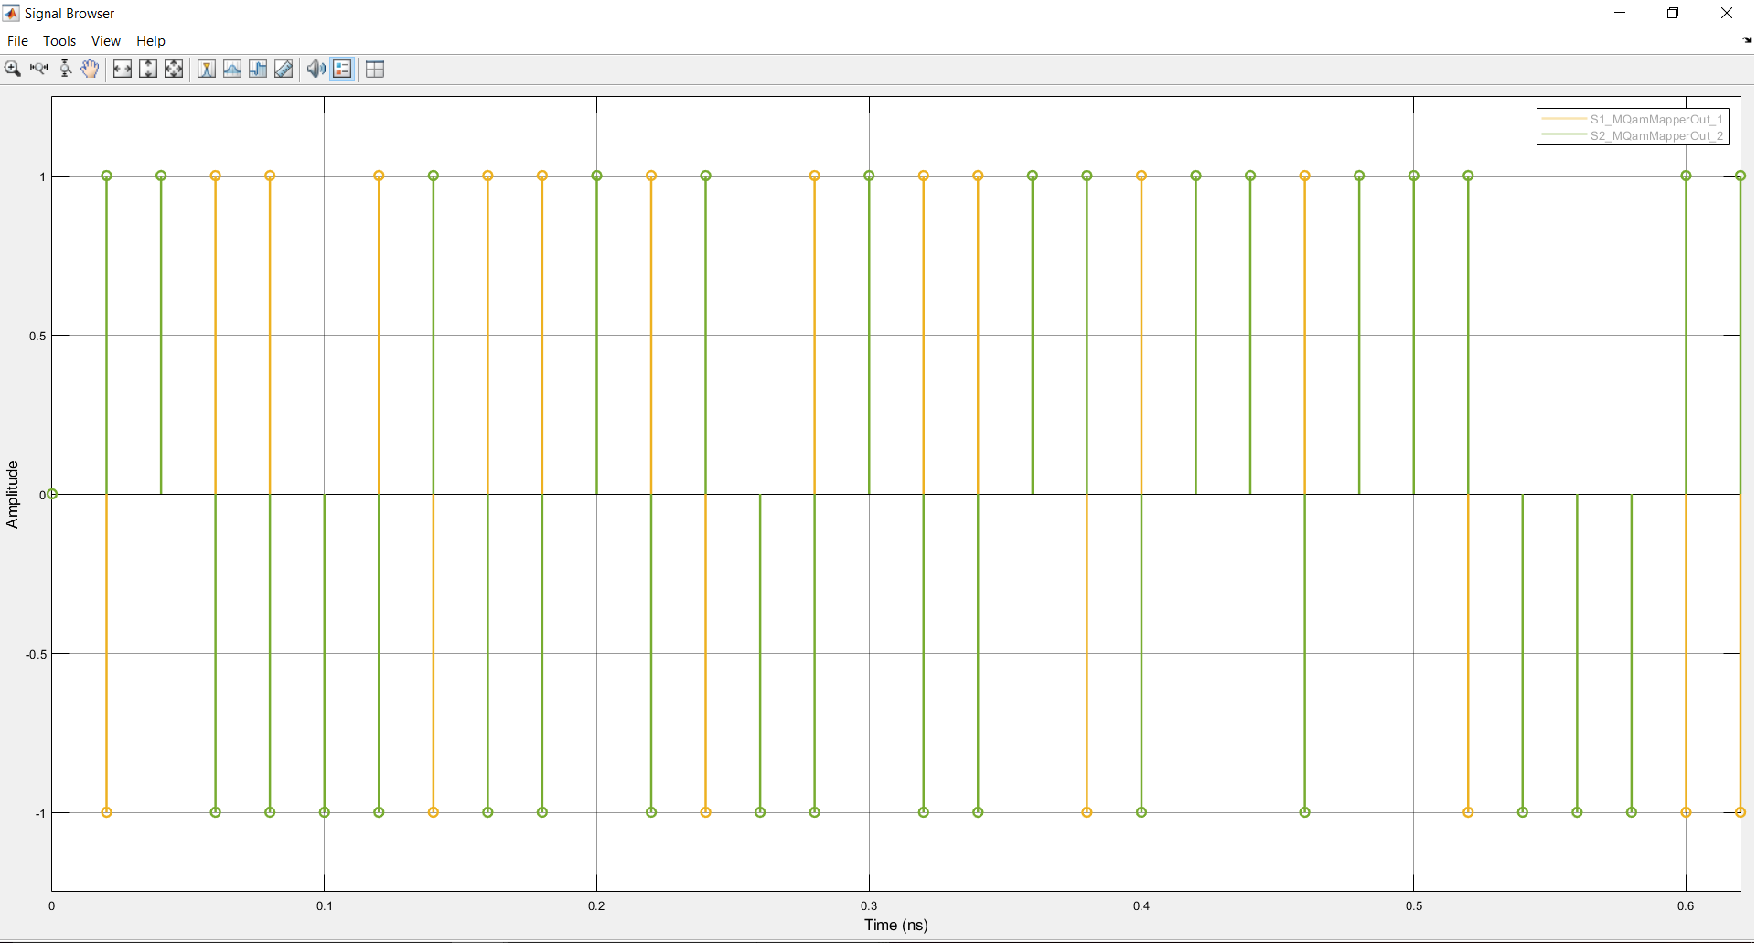
\includegraphics[width=1\textwidth]{../lib/discrete_to_continuous_time/figures/S1_S2.pdf}
	\caption{TimetoContinuous Input}\label{fig:TimetoContinuous Input}
\end{figure}

TimetoContinuous output:\\
S3(I): -1;1;1;1;-1;1;-1;1;1;1;1;-1;-1;1;1;1\\
S4(Q): 1;1;-1;-1;-1;-1;1;-1;-1;1;-1;1;-1;-1;1;-1\\
	
	\begin{figure}[h]
	\centering
	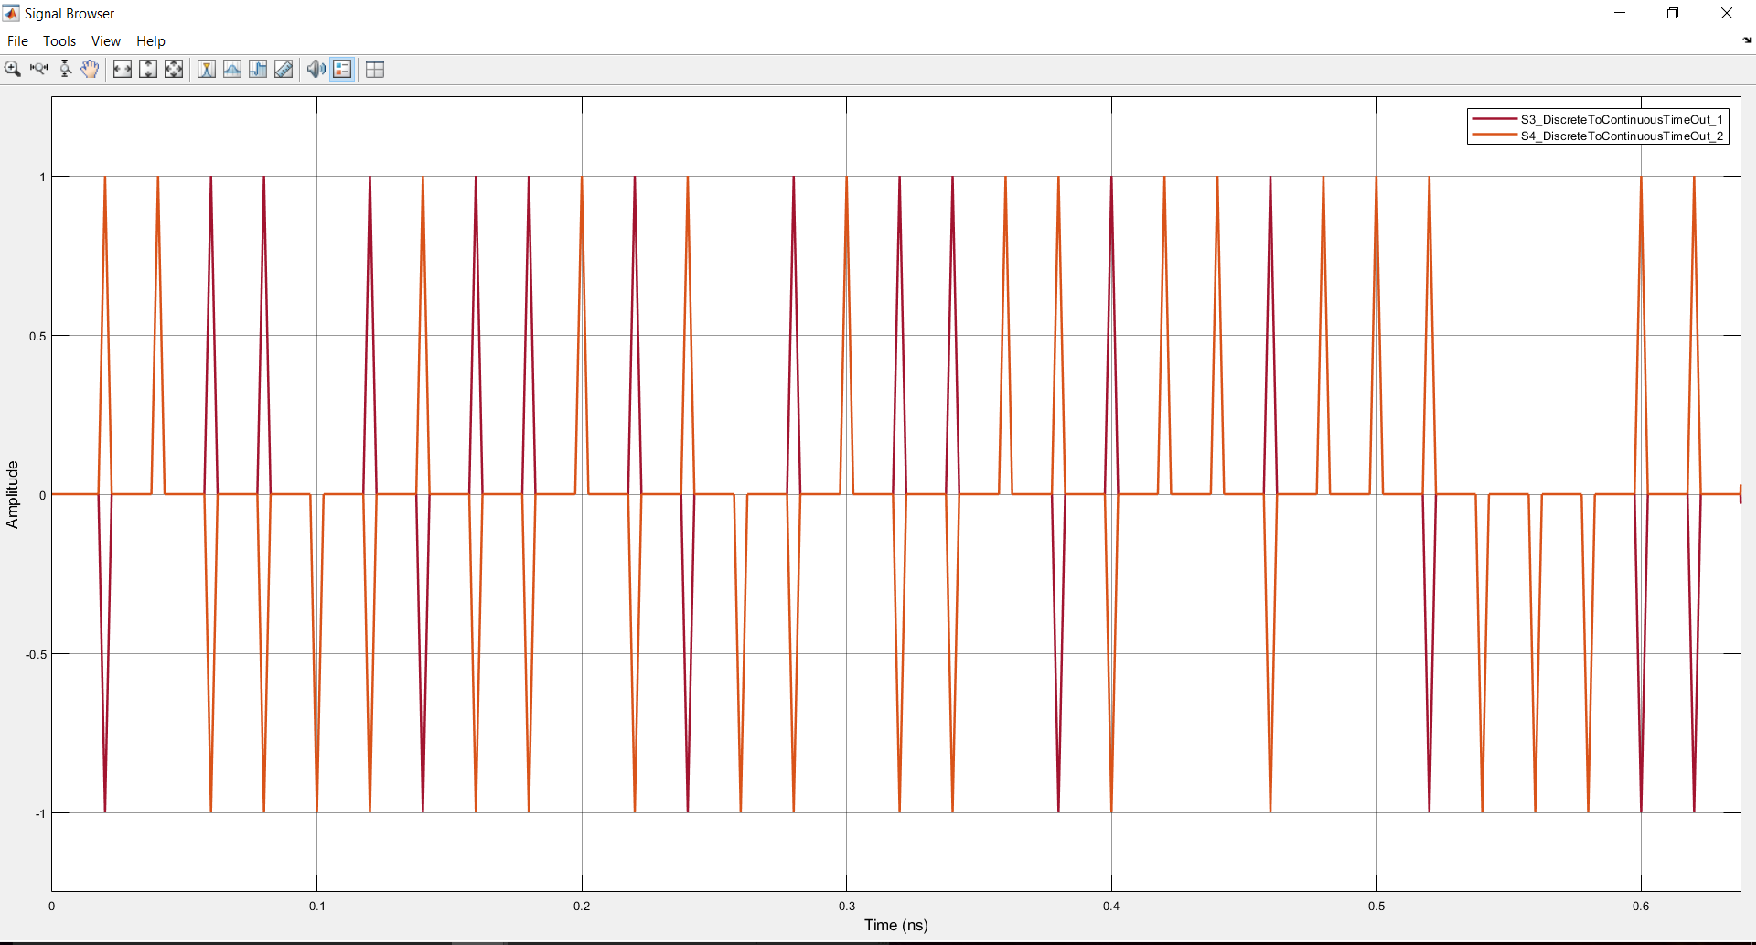
\includegraphics[width=1\textwidth]{../lib/discrete_to_continuous_time/figures/S3_S4.pdf}
	\caption{TimetoContinuous Output}\label{fig:TimetoContinuous Output}
\end{figure}

EyeDiagram:The open eye is large; IES=0;\\
	\begin{figure}[h]
	\centering
	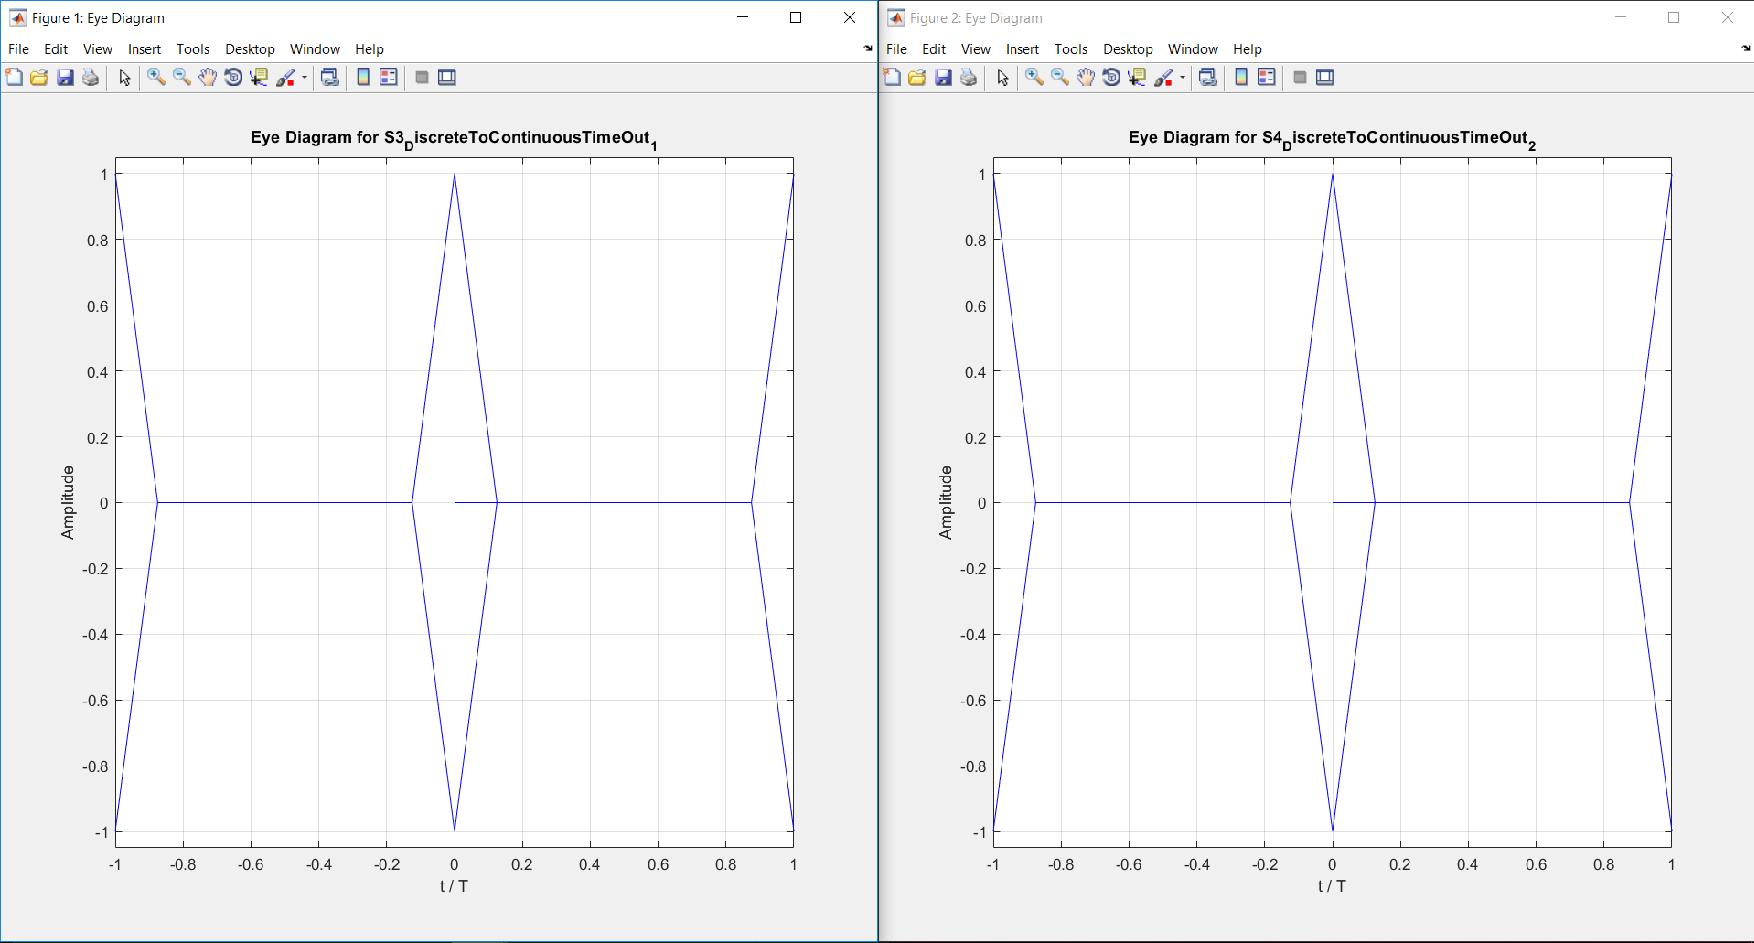
\includegraphics[width=1\textwidth]{../lib/discrete_to_continuous_time/figures/S3_S4_eye.pdf}
	\caption{Discrete To Continuous Time: Eye Diagram}\label{fig:TimetoContinuous : Eye Diagram}
\end{figure}

	
	
	

%\subsection*{Sugestions for future improvement}

\pagebreak
